\chapter{Работа с PKI} \label{chapt2}%
\textbf{Мета роботи:~}%
Изучить методы генерации простых чисел, проверку на простоту числа и
реализовать алгоритм ДХМ.
\section{Теоретические ведомости} \label{sect2_a}
% Лабораторная 2
Асимметричные криптографические системы были разработаны в 1970-х гг.
Принципиальное отличие асимметричной криптосистемы от криптосистемы
симметричного шифрования состоит в том, что для шифрования информации и её
последующей расшифровки используются различные ключи: открытый ключ К
\begin{Notes}
\item используется для шифрования информации, вычисляется из секретного ключа
    к;
\item секретный ключ к используется для расшифровки информации,
    зашифрованной с помощью парного ему открытого ключа К.
\end{Notes}

Эти ключи различаются таким образом, что с помощью вычислений нельзя вывести
секретный ключ к из открытого ключа К. Поэтому открытый ключ К может свободно
передаваться по каналам связи.
Асимметричные системы называют также
двухключевыми криптографическими системами, или криптосистемами с открытым
ключом.

Обобщенная схема асимметричной криптосистемы шифрования с открытым ключом
показана на \todo{рис ниже}
\begin{figure}[h]
  \centering
  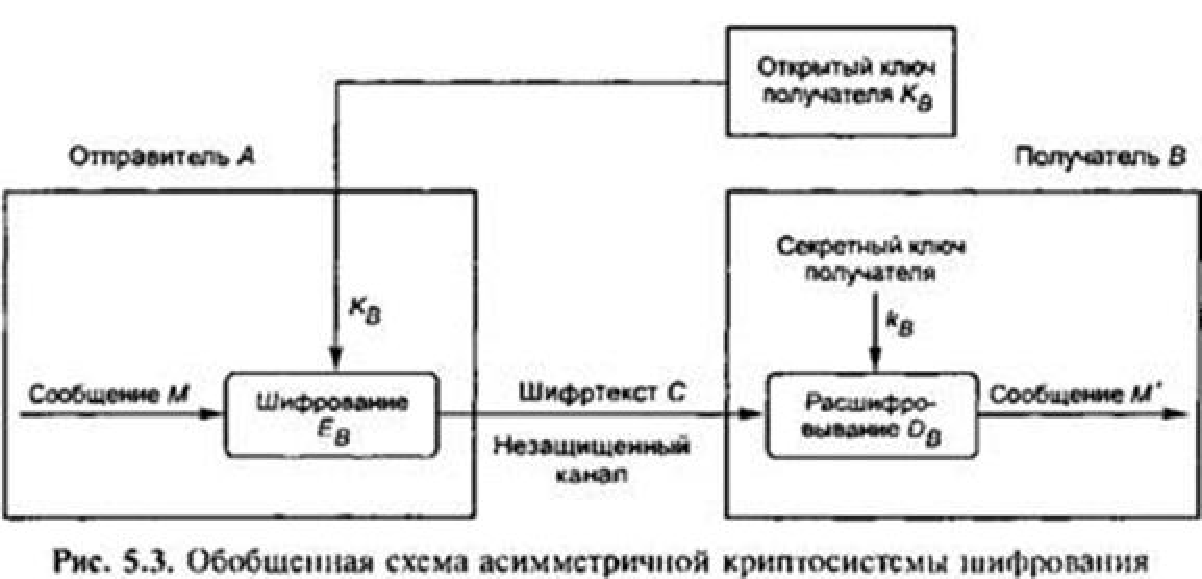
\includegraphics[width=\linewidth]{lab-2_1}
  \caption{Обобщённая схема асимметричной криптосистемы шифрования}\label{img:2_1}
\end{figure}

Для криптографического закрытия и последующего расшифровки передаваемой
информации используются открытый и секретный ключи получателя В сообщения. В
качестве ключа зашифровки должен использоваться открытый ключ получателя, а в
качестве ключа расшифровки — его секретный ключ.

Секретный и открытый ключи генерируются попарно. Секретный ключ должен
оставаться у его владельца и быть надежно защищен от НСД (аналогично ключу
шифрования в симметричных алгоритмах). Копия открытого ключа должна
находиться у каждого абонента криптографической сети, с которым обменивается
информацией владелец секретного ключа.

\paragraph{Передача ключа}
Процесс передачи зашифрованной информации в асимметричной криптосистеме
осуществляется следующим образом.

\subparagraph{Подготовительный этап}
\begin{itemize}
  \item абонент В генерирует пару ключей: секретный ключ кв и открытый ключ
      Кв;
  \item открытый ключ Кв посылается абоненту А и остальным абонентам (или
      делается доступным, например на разделяемом ресурсе).
\end{itemize}

\subparagraph{Обмен информацией между абонентами А и В}
\begin{itemize}
  \item абонент А шифрует сообщение с помощью открытого ключа Кв абонента В
      и отправляет шифротекст абоненту В;
  \item абонент В расшифровывает сообщение с помощью своего секретного
      ключа кв.
\end{itemize}
Никто другой (в том числе абонент А) не может расшифровать данное сообщение,
так как не имеет секретного ключа абонента В. Защита информации в
асимметричной криптосистеме основана на секретности ключа кв получателя
сообщения.

\subparagraph{Характерные особенности асимметричных криптосистем}
\begin{itemize}
  \item открытый ключ Кв и криптограмма С могут быть отправлены по
      незащищенным каналам, т. е. противнику известны Кв и С;
  \item  алгоритмы шифрования и расшифровывания: Ев : М → С; DB : С → М
      являются открытыми.
\end{itemize}
%
\paragraph{Методы генерации простых чисел}
%
Задача генерации простых чисел относится к классическим вычислительным
проблемам, известным с античных времен. С появлением криптографии с открытым
ключом эта проблема приобрела не только теоретическое, но и большое
практическое значение, так как большие случайные простые числа служат
параметрами (открытыми или закрытыми) многих асимметричных криптосистем.
Поскольку «формула» построения простого числа не известна (хотя её поисками
занимались многие выдающиеся математики), то все методы генерации простых
чисел действуют по следующей схеме: строится случайное нечетное число n
нужной длины и затем проверяется на простоту одним из известных тестов.

В 1976 г. Х. Уильямс привел следующую классификацию методов проверки чисел на
простоту (судя по более поздним публикациям, эта классификация не потеряла
актуальности по настоящее время):

Детерминированные методы, использующие специальные функции и/или знание
полного или частичного разложения числа n – 1 на простые множители. Эти
методы математически строго доказывают простоту или составность проверяемого
числа n. Методы Монте-Карло (вероятностные) – не требуют разложения на
простые множители, работают очень быстро, но не дают строгого доказательства
простоты (составности) числа. Методы гипотез – промежуточные между методами
Монте-Карло и математически строгими методами. Основаны на истинности
какой-либо недоказанной пока гипотезы (например, обобщённой гипотезы Римана):
в предположении, что гипотеза верна, эти методы превращаются в
детерминированные. Все детерминированные методы, которые были известны до
августа 2002 г., имеют экспоненциальную оценку сложности. В работе индийских
математиков M. Agrawal, N. Kayal, N. Saxena с замечательным названием
<<PRIMES is in P>> представлен детерминированный полиномиальный тест на
простоту; однако на данный момент вследствие своей сложности этот тест имеет
скорее теоретическое, чем практическое значение.

\paragraph{Известные алгоритмы}
%
\todo{Извесные алгоритмы сегодня}

\paragraph{Алгоритма Диффи-Хелмана}
%
\todo{История, цель и важность}

\subparagraph{Принцип работы алгоритма}

\todo{Отобразить принцип работы алгоритма}

\subparagraph{Пример реализации} блок схема(как там мороки много)

\section{Задания}\label{sect2_b}
%
Стандартный алгоритм для выполнения работы --- Алгоритм ДХМ. Не запрещено
использовать более новые алгоритмы, соответствующие тем же принципам что и
данный ДХМ.

Вариант задания указан в \todo{табл.}.

\noindent Уровень 1.

\begin{enumerate}
    \item Описать последовательность выполнения алгоритма для шифрования
        задания по варианту указаному выше.
  \item Исследовать использование алгоритма в различных сферах ИБ. Указать
      реальное применение данного алгоритма.
\end{enumerate}

\noindent Уровень 2.

\begin{enumerate}
  \item Составить программу для реализации алгоритма ДХМ.
  \item Произвести поэтапный обмен между двумя клиентами.
  \item Предоставить все промежуточные данные, как на \todo{табл.}
  \item Продемонстрировать шифрованный блок и записать его в отчёт.
\end{enumerate}

\noindent Уровень 3.

\begin{enumerate}
  \item Разработать приложение клиент-клиент обмена информацией между
      несколькими людьми. Используя асинхронный алгоритм шифрования.
  \item Продемонстрировать выполнение приложения.
  \item Предоставить исходный код в дополнение отчёта.
\end{enumerate}
Приложение может быть составлено в любом варианте, например: онлайн передача,
запись в шифрованный файл, почтовый шифр и другие.
\section{Пример выполнения работы}\label{sect2_c}
%
\section{Варианты}\label{sect2_d}
%
\section{Вопросы для контроля}\label{sect2_e}
\begin{enumerate}
  \item Асимметричные системы.
  \item Привести примеры асимметричных алгоритмов.
  \item Криптосистемы. Использование асимметричный алгоритмов.
  \item Преимущества и недостатки асимметричный систем.
  \item Методы подбора ключа в асимметричных криптосистемах.
  \item Сферы использование асимметричных алгоритмов.
  \item Описать однонаправленные функции. Привести примеры.
\end{enumerate}
%
